\documentclass{article}
\usepackage{fancyhdr}
\usepackage{multicol}
\usepackage{multirow}
\usepackage{booktabs}
\usepackage{pgfplots}
\pgfplotsset{compat=newest}
\usepackage[%
%A5,
    papersize={5.5in,8.5in},
    margin=0.75in,
    top=0.75in,
    bottom=0.75in,
%TWO SIDED
    ]{geometry}

\usepackage{xcolor}
\usepackage{graphicx}

\raggedcolumns
\setlength{\multicolsep}{0pt}
\setlength{\columnseprule}{1pt}

\makeatletter

\newif\if@mainmatter \@mainmattertrue

\newcommand\frontmatter{%
    \cleardoublepage
  \@mainmatterfalse
  \pagenumbering{roman}}
\newcommand\mainmatter{%
    \cleardoublepage
  \@mainmattertrue
  \pagenumbering{arabic}}
\makeatother

%DEFINE COLORS OF HEADER CLASSIFICATIONS HERE
\definecolor{gluten_color}{rgb}{0,0.5,0.2}
\definecolor{desert_color}{rgb}{0,0,1}
\definecolor{bread_color}{rgb}{0,0,1}
\definecolor{maincourse_color}{rgb}{0,0,1}
\definecolor{christmas_color}{rgb}{0,0,1}
\definecolor{easter_color}{rgb}{0,0,1}
\definecolor{soup_color}{rgb}{0,0,1}
\definecolor{preserves_color}{rgb}{0,0,1}
% START RECIPES.STY
\newcommand{\recipe}[2][]{%
    \newpage
    \lhead{}%
    \chead{}%
    \rhead{}%
    \lfoot{}%
    \rfoot{}%
    \section{#2}%
    \if###1##%
    \else
        \begin{center}
            \parbox{0.75\linewidth}{\raggedright\itshape#1}%
        \end{center}
    \fi
}
\newcommand{\serves}[2][Serves]{%
   \chead{#1 #2}}
\newcommand{\gluten}{%
    \rhead{\large\color{gluten_color}\textbf{GLUTEN}}}
\newcommand{\desert}{%
    \lhead{\large\color{desert_color}\textbf{DESERT}}}
\newcommand{\bread}{%
    \lhead{\large\color{bread_color}\textbf{BREAD}}}
\newcommand{\maincourse}{%
    \lhead{\large\color{maincourse_color}\textbf{MAIN COURSE}}}
\newcommand{\christmas}{%
    \lhead{\large\color{christmas_color}\textbf{CHRISTMAS}}}
\newcommand{\easter}{%
    \lhead{\large\color{easter_color}\textbf{EASTER}}}
\newcommand{\soup}{%
    \lhead{\large\color{soup_color}\textbf{SOUP}}}
\newcommand{\preserves}{%
    \lhead{\large\color{preserves_color}\textbf{PRESERVES}}}
%% Optional arguments for alternate names for these:
\newcommand{\preptime}[2][Prep]{%
    \lfoot{#1: #2}%
}
\newcommand{\cooktime}[2][Cook]{%
    \rfoot{#1: #2}%
}
\newcommand{\tempF}[1]{%
    $#1^\circ$F}
\newcommand{\tempC}[1]{%
    $#1^\circ$C}
%IMAGE GRAPHICS CONTROL
\newcommand{\showit}[3][1in]{%
    \begin{center}
        \bigskip
            \includegraphics[width=#1]{#2}%
            \par
            \medskip
            \emph{#3}
            \par
        \end{center}%
    }

\newcommand{\ingredients}[1][]{%
    \if###1##%
        {\color{red}\Large\textbf{Ingredients}}%
    \else
        \emph{#1}%
    \fi
}

\newenvironment{ingreds}{%
    \parindent0pt
    \noindent
    \ingredients
    \par
    \smallskip
    \begin{multicols}{2}
    \leftskip1em
    \rightskip0pt plus 3em
    \parskip=0.25em
    \obeylines
    \everypar={\hangindent2em}
}{%
    \end{multicols}%
    \medskip
}

\newcounter{stepnum}

\newenvironment{method}[1][]{%
    \setcounter{stepnum}{0}
    \noindent
    {\color{red}\Large\textbf{Step}}%
    \par
    \smallskip
    \if###1##%
    \else
        \noindent
        \emph{#1}
        \par
    \fi
    \begingroup
    \parindent0pt
    \parskip0.25em
        \leftskip2em
    \everypar={\llap{\stepcounter{stepnum}\hbox to2em{\thestepnum.\hfill}}}
}{%
    \par
    \endgroup}

\pagestyle{fancy}
% END RECIPES.STY

\begin{document}

\frontmatter
\tableofcontents

\mainmatter
%NEW RECIPE STARTS HERE. COPY AND PASTE TO BOTTOM OF DOCUMENT (BEFORE DOCUMENT END LINE) TO ADD ANOTHER RECIPE ITEM.
%%
%%
%%
%%
\recipe[A simple but elegant dessert pastry.]{Babka}
% LIST SERVING SIZE IN HEADER-CENTER
%\serves{4}
% LIST PREP TIME IN FOOTER-LEFT
\preptime{3 hour(s)}
%LIST COOK TIME IN FOOTER-RIGHT
%\cooktime [ADDING ANYTHING HERE WILL REPLACE COOK TIME TEXT, IE. CHILL, BAKE TIME, ETC.] {1 hour(s)}
\cooktime [BAKE] {1 hour(s)}
%RIGHT HEADER GLUTEN WARNING. COMMENT TO REMOVE
\gluten
%LEFT HEADER RECIPE TYPE LEAVE ONLY ONE CATEGORY NOT COMMENTED
\desert
%\bread
%\maincourse
%\christmas
%\easter
%\soup
%\preserves
\begin{ingreds}
%LEFT COLUMN
\ingredients[Dry:]
    120g whole wheat flour
    230g bread flour
    50g almond flour
    1tsp dry active yeast
\columnbreak
%RIGHT COLUMN
\ingredients[Wet:]
    2/3 cup warm milk
    2 eggs
    1/4 cup agave nectar
\ingredients[Other:]
    1 pinch salt
    1 stick butter
    90g starter
    1 handful dried cranberries
    1 handful dried raisins
\end{ingreds}

\begin{method}[Preheat oven at convection bake \tempF{325}.]
%NEW LINE WILL AUTO INCREMENT PARAGRAPH NUMBER
Mix the dry and wet ingredients separately.

Add the wet mix into the flour mix, add in the starter.

Mix until all flour is wet.

Rest for 20 minutes.

Knead the dough until tacky, not sticky.

Knead in butter.

Knead in dried fruit.

Cover and let rise up to 2 hours.

Shape and proof up to 2 hours.

Bake at convection \tempF{325} for 30 minutes.
\end {method}
%OPTIONAL IMAGE TO ATTACH
%\showit[1.25in]{example-image-b}{image description}
%%
%%
%%
%%
\recipe[Bread recipe description.]{Bread}
% LIST SERVING SIZE IN HEADER-CENTER
%\serves{4}
% LIST PREP TIME IN FOOTER-LEFT
%\preptime{3 hour(s)}
%LIST COOK TIME IN FOOTER-RIGHT
%\cooktime [ADDING ANYTHING HERE WILL REPLACE COOK TIME TEXT, IE. CHILL, BAKE TIME, ETC.] {1 hour(s)}
%\cooktime [BAKE] {1 hour(s)}
%RIGHT HEADER GLUTEN WARNING. COMMENT TO REMOVE
\gluten
%LEFT HEADER RECIPE TYPE LEAVE ONLY ONE CATEGORY NOT COMMENTED
%\desert
\bread
%\maincourse
%\christmas
%\easter
%\soup
%\preserves
\begin{ingreds}
%LEFT COLUMN
\ingredients[WHITE:]
810g water
150g starter
70g wheat germ
200g whole wheat flour
\columnbreak
%RIGHT COLUMN
\ingredients[RYE:]
810g water
150g starter
70g wheat germ
150g dark rye flour
100g whole wheat
\end{ingreds}

\begin{method}[If white, wet all ingredients, mix in 800g bread flour. If Rye, wet all ingredients, rest for 1 hour, mix in 750g bread flour. Then:]
%NEW LINE WILL AUTO INCREMENT PARAGRAPH NUMBER
Let rest for 30 minutes.

Add 20g salt, 60g water (50g if ambient temperature $\geq$\tempF{85}).

Add seeds with salt during the first flip.

If rise in the fridge, put the dough in the fridge after everything is incorporated. If rise at room temperature flip every 30 minutes during the first 2 hours.

Rest for another 2 hours (1 hour if temperature $\geq$\tempF {80}).

Divide each batch of dough by two for 2lbs loaves (by four for 1lb loaves).

Shape and refrigerate overnight, or 8 hours.

Warm up oven with steam to \tempF{500}.

Baking profile:
\begin{tabular}{lll}
\hline
\textbf{Type}          & \textbf{Temp} & \textbf{Time}  \\
\hline
\multirow{3}{*}{White} & 500           & 8              \\
                       & 425           & 30             \\
                       & Coast         & 6              \\
\hline
\multirow{2}{*}{Rye}   & 425           & 40             \\
                       & Coast         & 6              \\
\hline
\multicolumn{3}{l}{Skip coasting for small loaves.}
\end{tabular}

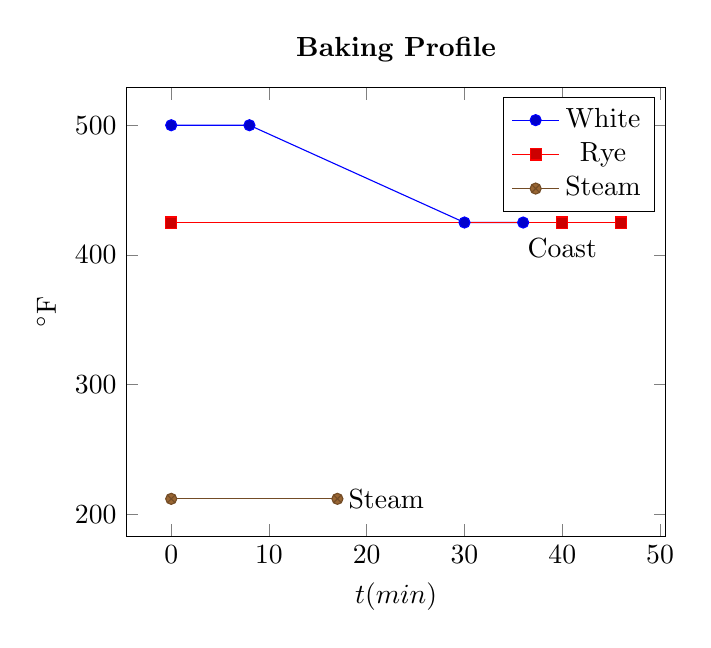
\begin{tikzpicture}
\begin{axis}[
title={\textbf{Baking Profile}}
,xlabel={$t(min)$}
,ylabel={$\tempF$}]
domain=0:60
,ymin=200
,ymax=525
%,legend pos={south east}
\addplot+  plot coordinates
{ (0,500) (8,500) (30,425) (36,425)};
\addlegendentry{White}
\addplot+ plot coordinates
%\node[circle,fill=blue,scale=0.5,pin=135:{$(40,425)$}];
{ (0,425) (40,425) (46,425)};
\node at (axis cs:40,405) {Coast};
\addlegendentry{Rye}
\addplot+ plot coordinates
{ (0,212) (17,212)};
\node at (axis cs:22,212) {Steam};
\addlegendentry{Steam}
\end{axis}
\end{tikzpicture}

Turn off the steam after 17 minutes.

Rotate loaves half way through.

If using Dutch oven, ramp down:
\begin{description}
  \item[1lb loaf]\tempF{500} to \tempF{425} in steps of \tempF{25} every 5 minutes;
  \item[2lbs loaf]\tempF{500} to \tempF{425} in steps of \tempF{25} every 7 minutes;
  \item[3lbs loaf]\tempF{500} to \tempF{425} in steps of \tempF{25} every 10 minutes;
\end{description}
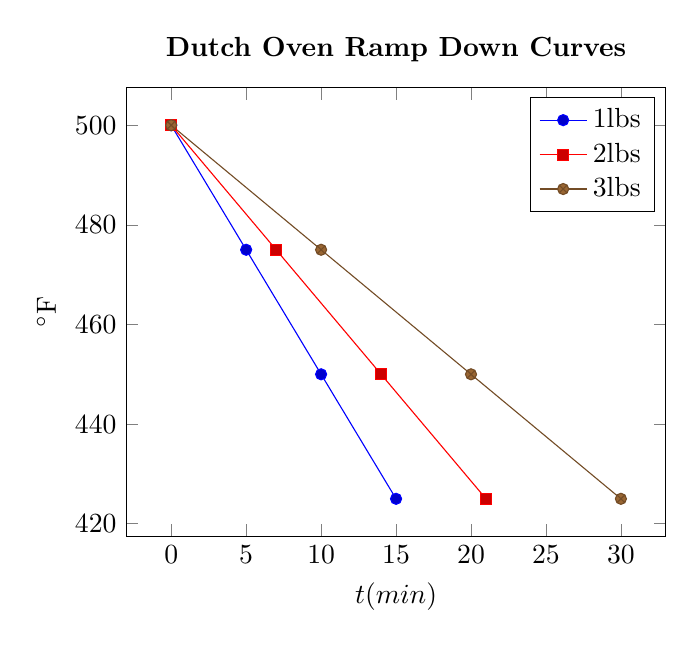
\begin{tikzpicture}
\begin{axis}[title={\textbf{Dutch Oven Ramp Down Curves}},
xlabel={$t(min)$}, ylabel={$\tempF$}]
domain=0:30, ymin=400, ymax=525
\addplot+[smooth] plot coordinates
{ (0,500) (5,475) (10,450) (15,425)};
\addlegendentry{1lbs}
\addplot+[smooth] plot coordinates
{ (0,500) (7,475) (14,450) (21,425)};
\addlegendentry{2lbs}
\addplot+[smooth] plot coordinates
{ (0,500) (10,475) (20,450) (30,425)};
\addlegendentry{3lbs}
\end{axis}
\end{tikzpicture}
Remove Dutch oven lid at \tempF{425}, bake for additional 20 min (30 min for 3lbs loaf).
\end {method}
\begin{method}[Preheat Dutch oven to \tempF{500}. Bake at \tempF{425} for 40 minutes.]
\begin{tabular}{l|lll}
\multicolumn{1}{l}{\textbf{}} & \textbf{Water(g)} & \textbf{Rye(g)} & \textbf{Seeds(g)}  \\
\hline
\textbf{Starter}                        & 125            & 100          &                 \\
\textbf{Soaker, rye}                    & 100            & 100          &                 \\
\textbf{Soaker, seeds}                  & 60             &              & 150             \\
\textbf{Final dough}                    & 215            & 200          &                 \\
\textbf{Total}                          & 500            & 400          &
\end{tabular}

\end{method}


%OPTIONAL IMAGE TO ATTACH
%\showit[1.25in]{example-image-b}{image description}
%%
%%
%%
%%
\end{document} 